\documentclass[aspectratio=169,10pt]{beamer}
\usetheme{Madrid}
\usecolortheme{default}

\usepackage{hyperref}
\usepackage{tikz}
\usetikzlibrary{patterns,shapes,arrows,calc,positioning,decorations.markings}
\usepackage{circuitikz}
\usepackage{amsmath,amssymb}
\usepackage{graphicx}
\usepackage{listings}
\usepackage{booktabs}

% --- Custom Colors UNIB ---
\definecolor{unibblue}{RGB}{0, 32, 96}
\definecolor{unibgold}{RGB}{197, 160, 89}
\definecolor{unibgreen}{RGB}{34, 112, 60}

\setbeamercolor{palette primary}{bg=unibblue,fg=white}
\setbeamercolor{palette secondary}{bg=unibblue!85,fg=white}
\setbeamercolor{palette tertiary}{bg=unibblue!70,fg=white}
\setbeamercolor{structure}{fg=unibblue}
\setbeamercolor{titlelike}{parent=structure,bg=unibblue,fg=white}
\setbeamercolor{block title}{bg=unibblue!90,fg=white}
\setbeamercolor{block body}{bg=unibblue!8,fg=black}
\setbeamercolor{alertblock title}{bg=unibgold!95,fg=black}
\setbeamercolor{alertblock body}{bg=unibgold!15,fg=black}
\setbeamercolor{exampleblock title}{bg=unibgreen!90,fg=white}
\setbeamercolor{exampleblock body}{bg=unibgreen!10,fg=black}

% --- Pengaturan Listing Julia ---
\lstdefinelanguage{Julia}%
  {morekeywords={abstract,break,case,catch,const,continue,do,else,elseif,%
      end,export,false,for,function,global,if,import,%
      let,local,macro,module,mutable,primitive,quote,return,struct,%
      true,try,type,using,var,while},%
   sensitive=true,%
   morecomment=[l]{\#},%
   morecomment=[n]{\#=}{=\#},%
   morestring=[b]',%
   morestring=[b]"%
  }[keywords,comments,strings]

\lstdefinestyle{juliastyle}{
    language=Julia,
    basicstyle=\ttfamily\tiny,
    keywordstyle=\color{blue!80!black}\bfseries,
    commentstyle=\color{green!50!black}\itshape,
    stringstyle=\color{red!80!black},
    numbers=none,
    breaklines=true,
    showstringspaces=false,
    frame=single,
    backgroundcolor=\color{gray!6},
    xleftmargin=4pt,
    xrightmargin=4pt,
    aboveskip=2pt,
    belowskip=2pt
}

\title[Persamaan Diferensial (Minggu 6)]{Persamaan Diferensial}
\subtitle{Minggu 6: Transformasi Laplace Dasar \& Teorema Pergeseran Domain-s}
\author[Novalio \& Arfan (UNIB)]{Ir. Novalio Daratha, S.T., M.Sc., Ph.D. \& Muhammad Arfan, S.T., M.T.}
\institute[Teknik Elektro UNIB]{Program Studi S1 Teknik Elektro, Jurusan Teknik Elektro \& Informatika\\Fakultas Teknik, Universitas Bengkulu}
\date[2026]{Semester Genap 2026 \\[1.5mm] {\scriptsize\color{red!85!black}\textbf{Video Kuliah:}} {\scriptsize\url{https://youtu.be/iIYM-WRaTiU}} \quad \textbar \quad {\scriptsize\href{https://www.youtube.com/playlist?list=PLS5oOZWXZeTw}{\color{unibblue}\textbf{Playlist YouTube}}}}

\begin{document}

% FRAME 1: Titlepage
\begin{frame}[plain]
  \titlepage
\end{frame}

% FRAME 2: Sub-CPMK OBE Bloom
\begin{frame}{Capaian Pembelajaran (Sub-CPMK 4) \& Taksonomi Bloom}
  \begin{block}{Sub-CPMK Minggu 6 (Transformasi Laplace \& Sinyal Diskontinu)}
    Mahasiswa mampu memetakan fungsi waktu ke domain frekuensi kompleks $s$, menerapkan sifat kelinieran dan teorema translasi, memodelkan sinyal pensaklaran Heaviside dan surja impuls Dirac, serta mentransformasikan PDB orde 2 menjadi persamaan aljabar.
  \end{block}
  \vspace{0.15cm}
  \begin{columns}[t]
    \column{0.5\textwidth}
    \textbf{Target Kognitif (Bloom C1--C3):}
    \begin{itemize}
      \item \textbf{C1 (Mengingat):} Menyatakan definisi integral Laplace dan pasangan fungsi baku ($1, t^n, e^{at}, \sin, \cos$).
      \item \textbf{C2 (Memahami):} Menjelaskan peran fungsi tangga Heaviside $u(t)$ dan impuls Dirac $\delta(t)$ dalam elektro.
      \item \textbf{C3 (Menerapkan):} Menghitung transformasi menggunakan Teorema Pergeseran Pertama dan Kedua.
    \end{itemize}

    \column{0.5\textwidth}
    \textbf{Target Kognitif (Bloom C4--C6):}
    \begin{itemize}
      \item \textbf{C4 (Menganalisis):} Mentransformasikan operator turunan PDB lengkap dengan syarat awal IVP.
      \item \textbf{C5 (Mengevaluasi):} Menganalisis respon surja petir standar IEC 60060-1 ($1{,}2/50\,\mu\text{s}$) pada isolasi gardu PLN.
      \item \textbf{C6 (Komputasi):} Memprogram visualisasi medan kutub-nol (\textit{pole-zero map}) pada bidang-$s$ dengan Julia.
    \end{itemize}
  \end{columns}
\end{frame}

% FRAME 3: Peta Konsep Laplace
\begin{frame}{Peta Konsep: Mengapa Beralih ke Domain Kompleks $s$?}
  \begin{center}
    \resizebox{0.92\linewidth}{!}{%
    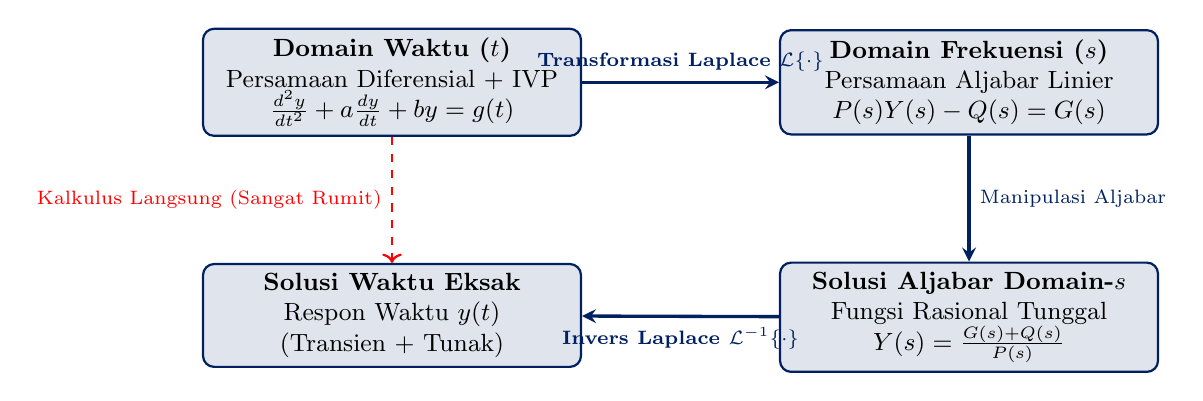
\begin{tikzpicture}[
      node distance=1.5cm and 2.5cm,
      block/.style={rectangle, draw=unibblue, fill=unibblue!12, thick, rounded corners, align=center, font=\small, minimum width=4.8cm, minimum height=1.1cm},
      arrow/.style={->, >=stealth, very thick, unibblue}
    ]
      \node[block] (t_diff) {\textbf{Domain Waktu ($t$)}\\Persamaan Diferensial + IVP\\$\frac{d^2 y}{dt^2} + a \frac{dy}{dt} + b y = g(t)$};
      \node[block, right=of t_diff] (s_alg) {\textbf{Domain Frekuensi ($s$)}\\Persamaan Aljabar Linier\\$P(s) Y(s) - Q(s) = G(s)$};
      \node[block, below=1.6cm of t_diff] (t_sol) {\textbf{Solusi Waktu Eksak}\\Respon Waktu $y(t)$\\(Transien + Tunak)};
      \node[block, below=1.6cm of s_alg] (s_sol) {\textbf{Solusi Aljabar Domain-$s$}\\Fungsi Rasional Tunggal\\$Y(s) = \frac{G(s) + Q(s)}{P(s)}$};

      \draw[arrow] (t_diff) -- node[above, font=\scriptsize\bfseries] {Transformasi Laplace $\mathcal{L}\{\cdot\}$} (s_alg);
      \draw[arrow] (s_alg) -- node[right, font=\scriptsize] {Manipulasi Aljabar} (s_sol);
      \draw[arrow] (s_sol) -- node[below, font=\scriptsize\bfseries] {Invers Laplace $\mathcal{L}^{-1}\{\cdot\}$} (t_sol);
      \draw[dashed, red, ->, thick] (t_diff) -- node[left, font=\scriptsize] {Kalkulus Langsung (Sangat Rumit)} (t_sol);
    \end{tikzpicture}%
    }
  \end{center}
\end{frame}

% FRAME 4: Definisi Formal Transformasi Laplace
\begin{frame}{Definisi Formal \& Syarat Keberadaan Transformasi Laplace}
  \begin{block}{Definisi Integral Laplace Unilateral}
    Transformasi Laplace dari fungsi waktu $f(t)$ yang terdefinisi untuk $t \ge 0$ didefinisikan sebagai integral tak wajar:
    \begin{equation}
      \mathbf{\mathcal{L}\{f(t)\} = F(s) = \int_0^\infty f(t) e^{-st} dt}
    \end{equation}
    di mana $s = \sigma + j\omega$ adalah variabel frekuensi kompleks.
  \end{block}
  \vspace{0.15cm}
  \begin{alertblock}{Syarat Keberadaan (\textit{Existence Condition})}
    Integral konvergen di wilayah konvergensi (\textit{ROC}) jika $f(t)$ memenuhi:
    \begin{enumerate}
      \item Kontinu sepotong demi sepotong (\textit{piecewise continuous}) pada setiap interval $[0, T]$.
      \item Berorde eksponensial (\textit{exponential order}): $|f(t)| \le M e^{\gamma t}$ untuk semua $t \ge t_0$.
    \end{enumerate}
  \end{alertblock}
\end{frame}

% FRAME 5: Pasangan Transformasi Baku
\begin{frame}{Pasangan Transformasi Laplace Baku Fungsi Elementer}
  \begin{center}
    \small
    \begin{tabular}{lllc}
      \toprule
      \textbf{Fungsi Domain Waktu $f(t)$} & \textbf{Transformasi $F(s) = \mathcal{L}\{f(t)\}$} & \textbf{Wilayah Konvergensi (ROC)} \\ \midrule
      Konstanta / Tangga Satuan: $1$ atau $u(t)$ & $\mathbf{\frac{1}{s}}$ & $\text{Re}(s) > 0$ \\
      Pangkat: $t^n$ ($n \in \mathbb{N}$) & $\mathbf{\frac{n!}{s^{n+1}}}$ & $\text{Re}(s) > 0$ \\
      Eksponensial: $e^{at}$ & $\mathbf{\frac{1}{s - a}}$ & $\text{Re}(s) > a$ \\
      Sinusoidal: $\sin(\omega t)$ & $\mathbf{\frac{\omega}{s^2 + \omega^2}}$ & $\text{Re}(s) > 0$ \\
      Cosinusoidal: $\cos(\omega t)$ & $\mathbf{\frac{s}{s^2 + \omega^2}}$ & $\text{Re}(s) > 0$ \\
      Impuls Satuan: $\delta(t)$ & $\mathbf{1}$ & Seluruh bidang-$s$ \\ \bottomrule
    \end{tabular}
  \end{center}
  \vspace{0.15cm}
  \footnotesize Seluruh kombinasi fungsi eksitasi teknik elektro dapat didekomposisi dari tabel pasangan dasar di atas.
\end{frame}

% FRAME 6: Linieritas & Transformasi Turunan
\begin{frame}{Sifat Linieritas \& Transformasi Operator Turunan}
  \begin{columns}[t]
    \column{0.48\textwidth}
    \begin{block}{Sifat Kelinieran}
      \begin{equation*}
        \mathcal{L}\{c_1 f_1(t) + c_2 f_2(t)\} = c_1 F_1(s) + c_2 F_2(s)
      \end{equation*}
      Memungkinkan pemecahan sinyal kompleks menjadi jumlahan komponen sederhana.
    \end{block}

    \column{0.52\textwidth}
    \begin{alertblock}{Teorema Transformasi Turunan}
      \textbf{Turunan Pertama:}
      \begin{equation*}
        \mathbf{\mathcal{L}\{f'(t)\} = s F(s) - f(0^-)}
      \end{equation*}
      \textbf{Turunan Kedua:}
      \begin{equation*}
        \mathbf{\mathcal{L}\{f''(t)\} = s^2 F(s) - s f(0^-) - f'(0^-)}
      \end{equation*}
    \end{alertblock}
  \end{columns}
  \vspace{0.2cm}
  \textbf{Keunggulan Mutlak:} Syarat awal Masalah Nilai Awal (IVP) langsung terintegrasi secara otomatis ke dalam persamaan aljabar tanpa perlu mencari konstanta integrasi secara terpisah!
\end{frame}

% FRAME 7: Fungsi Khusus Heaviside
\begin{frame}{Fungsi Khusus 1: Tangga Satuan Heaviside $u(t - a)$}
  \begin{columns}[c]
    \column{0.52\textwidth}
    \textbf{Representasi Matematika Pensaklaran:}
    \begin{equation}
      u(t - a) = \begin{cases} 0, & t < a \\ 1, & t \ge a \end{cases}
    \end{equation}
    \begin{itemize}
      \item Memodelkan penutupan sakelar pada $t = a$.
      \item \textbf{Pulsa Segi Empat}: Sakelar on pada $t=a$ dan off pada $t=b$:
      \begin{equation*}
        p(t) = V_0 [u(t - a) - u(t - b)]
      \end{equation*}
      \item Transformasi Laplace:
      \begin{equation*}
        \mathbf{\mathcal{L}\{u(t - a)\} = \frac{e^{-as}}{s}}
      \end{equation*}
    \end{itemize}

    \column{0.44\textwidth}
    \begin{center}
      \resizebox{\linewidth}{!}{%
      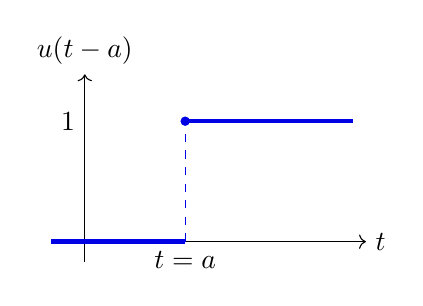
\begin{tikzpicture}[scale=0.85]
        \draw[->] (-0.5,0) -- (4.2,0) node[right] {$t$};
        \draw[->] (0,-0.3) -- (0,2.5) node[above] {$u(t-a)$};
        \draw[blue!90!black, ultra thick] (-0.5,0) -- (1.5,0);
        \draw[dashed, blue!90!black] (1.5,0) -- (1.5,1.8);
        \draw[blue!90!black, ultra thick] (1.5,1.8) -- (4.0,1.8);
        \fill[blue!90!black] (1.5,1.8) circle (2pt);
        \node[below] at (1.5,0) {$t = a$};
        \node[left] at (0,1.8) {$1$};
      \end{tikzpicture}%
      }
    \end{center}
  \end{columns}
\end{frame}

% FRAME 8: Fungsi Khusus Dirac
\begin{frame}{Fungsi Khusus 2: Impuls Satuan Dirac $\delta(t - a)$}
  \begin{columns}[c]
    \column{0.52\textwidth}
    \textbf{Representasi Kejutan Sesaat:}
    \begin{equation}
      \delta(t - a) = 0 \quad \forall t \neq a, \quad \int_{-\infty}^\infty \delta(t - a) dt = 1
    \end{equation}
    \begin{itemize}
      \item Turunan dari fungsi tangga: $\mathbf{\delta(t) = \frac{du(t)}{dt}}$.
      \item \textbf{Sifat Penyaringan (\textit{Sifting Property}):}
      \begin{equation*}
        \int_0^\infty f(t) \delta(t - a) dt = f(a)
      \end{equation*}
      \item Transformasi Laplace Impuls:
      \begin{equation*}
        \mathbf{\mathcal{L}\{\delta(t - a)\} = e^{-as} \implies \mathcal{L}\{\delta(t)\} = 1}
      \end{equation*}
    \end{itemize}

    \column{0.44\textwidth}
    \begin{alertblock}{Aplikasi dalam Elektro}
      Memodelkan sambaran kilat surja petir, pelepasan muatan elektrostatik (ESD), atau lonjakan switching berenergi tinggi dalam waktu mikrodetik.
    \end{alertblock}
  \end{columns}
\end{frame}

% FRAME 9: Teorema Pergeseran Pertama
\begin{frame}{Teorema Pergeseran Pertama (Translasi Frekuensi Sumbu-$s$)}
  \begin{block}{Teorema Translasi Sumbu-$s$}
    Jika $\mathcal{L}\{f(t)\} = F(s)$, maka perkalian dengan fungsi eksponensial $e^{at}$ di domain waktu menggeser variabel domain frekuensi sebesar $a$:
    \begin{equation}
      \mathbf{\mathcal{L}\{e^{at} f(t)\} = F(s - a)}
    \end{equation}
  \end{block}
  \vspace{0.15cm}
  \textbf{Aplikasi pada Bentuk Gelombang Teredam:}
  \begin{itemize}
    \item Sinusoidal Teredam:
    \begin{equation*}
      \mathcal{L}\{e^{-\alpha t} \sin\omega t\} = \left. \frac{\omega}{s^2 + \omega^2} \right|_{s \to s + \alpha} = \mathbf{\frac{\omega}{(s + \alpha)^2 + \omega^2}}
    \end{equation*}
    \item Cosinusoidal Teredam:
    \begin{equation*}
      \mathcal{L}\{e^{-\alpha t} \cos\omega t\} = \left. \frac{s}{s^2 + \omega^2} \right|_{s \to s + \alpha} = \mathbf{\frac{s + \alpha}{(s + \alpha)^2 + \omega^2}}
    \end{equation*}
  \end{itemize}
\end{frame}

% FRAME 10: Teorema Pergeseran Kedua
\begin{frame}{Teorema Pergeseran Kedua (Translasi Waktu Sumbu-$t$)}
  \begin{block}{Teorema Translasi Sumbu-$t$}
    Jika suatu sinyal $f(t)$ mengalami penundaan (\textit{delay}) sebesar $a > 0$ dan dinonaktifkan untuk $t < a$, transformasinya dikalikan dengan faktor eksponensial $e^{-as}$:
    \begin{equation}
      \mathbf{\mathcal{L}\{f(t - a) u(t - a)\} = e^{-as} F(s)}
    \end{equation}
  \end{block}
  \vspace{0.15cm}
  \begin{columns}[t]
    \column{0.5\textwidth}
    \textbf{Contoh Sinyal Pulsa Tegangan:}
    Pulsa tegangan $V_0$ dengan durasi aktif dari $t = t_1$ hingga $t = t_2$:
    \begin{equation*}
      v(t) = V_0 [u(t - t_1) - u(t - t_2)]
    \end{equation*}

    \column{0.5\textwidth}
    \begin{exampleblock}{Transformasi Laplace Pulsa}
      \begin{equation*}
        \mathbf{V(s) = \frac{V_0}{s} \left( e^{-t_1 s} - e^{-t_2 s} \right)}
      \end{equation*}
      Sangat praktis untuk analisis respons kendali inverter switching PWM!
    \end{exampleblock}
  \end{columns}
\end{frame}

% FRAME 11: Aplikasi Surja Petir IEC
\begin{frame}{Aplikasi Industri: Surja Petir Standar IEC 60060-1 / IEEE Std 4}
  \begin{columns}[c]
    \column{0.55\textwidth}
    \textbf{Model Matematis Surja Petir $1{,}2/50\,\mu\text{s}$:}
    \begin{itemize}
      \item Surja impuls petir pada gardu induk dimodelkan sebagai selisih dua fungsi eksponensial:
      \begin{equation}
        v_{\text{petir}}(t) = V_{\text{peak}} \cdot k \left( e^{-\alpha t} - e^{-\beta t} \right) u(t)
      \end{equation}
      dengan $\alpha \approx 1{,}46 \times 10^4\text{ s}^{-1}$ (ekor $50\,\mu\text{s}$) dan $\beta \approx 2{,}47 \times 10^6\text{ s}^{-1}$ (muka $1{,}2\,\mu\text{s}$).
      \item \textbf{Representasi Domain-$s$:}
      \begin{equation*}
        \mathbf{V(s) = V_{\text{peak}} \cdot k \left( \frac{1}{s + \alpha} - \frac{1}{s + \beta} \right)}
      \end{equation*}
    \end{itemize}

    \column{0.45\textwidth}
    \begin{alertblock}{Ketahanan Isolasi Gardu PLN}
      Transformator daya 150 kV harus memiliki nilai \textit{Basic Insulation Level} (BIL) minimal $650\text{ kV}$ untuk menahan tegangan impuls petir ini.
    \end{alertblock}
  \end{columns}
\end{frame}

% FRAME 12: Worked Example Konversi IVP ke Domain-s
\begin{frame}{Contoh Soal Terhitung (Worked Example): Konversi IVP ke Domain-$s$}
  \textbf{Soal:} Konversikan IVP $y'' + 4y' + 13y = 26 u(t)$ dengan $y(0^-) = 2, y'(0^-) = -1$ ke domain-$s$.
  \vspace{0.15cm}

  \begin{columns}[t]
    \column{0.48\textwidth}
    \textbf{1. Terapkan Teorema Turunan:}
    \begin{align*}
      \mathcal{L}\{y''\} &= s^2 Y(s) - 2s + 1 \\
      \mathcal{L}\{y'\}  &= s Y(s) - 2 \\
      \mathcal{L}\{y\}   &= Y(s) \\
      \mathcal{L}\{26 u(t)\} &= \frac{26}{s}
    \end{align*}
    \textbf{2. Substitusikan ke Persamaan:}
    \begin{equation*}
      [s^2 Y - 2s + 1] + 4[s Y - 2] + 13 Y = \frac{26}{s}
    \end{equation*}

    \column{0.48\textwidth}
    \textbf{3. Kelompokkan Suku $Y(s)$:}
    \begin{align*}
      (s^2 + 4s + 13) Y(s) - 2s - 7 &= \frac{26}{s} \\
      (s^2 + 4s + 13) Y(s) &= 2s + 7 + \frac{26}{s} \\
                           &= \frac{2s^2 + 7s + 26}{s}
    \end{align*}
    \textbf{4. Solusi Aljabar Akhir:}
    \begin{equation*}
      \mathbf{Y(s) = \frac{2s^2 + 7s + 26}{s(s^2 + 4s + 13)}}
    \end{equation*}
  \end{columns}
\end{frame}

% FRAME 13: Praktikum Komputasi Julia
% FRAME 13: Praktikum Komputasi Julia
\begin{frame}[fragile]{Praktikum Komputasi Julia: Surja Petir IEC 60060-1}
  \begin{columns}[t]
    \column{0.50\textwidth}
    \begin{block}{Skrip Julia: Gelombang Impuls Surja}
\begin{lstlisting}[style=juliastyle]
using Plots

t_us = range(0, 100, length=400)
alpha, beta = 0.0146e6, 2.467e6
V0 = 1.037

v_surge = @. V0 * (exp(-alpha * t_us * 1e-6) - exp(-beta * t_us * 1e-6))
plot(t_us, v_surge, lw=2, color=:red, label="1.2/50 us")
scatter!([1.2], [1.0], color=:blue, label="Puncak tp")
scatter!([50.0], [0.5], color=:green, label="Ekor t2")
\end{lstlisting}
    \end{block}

    \column{0.48\textwidth}
    \begin{alertblock}{Visualisasi Surja Petir Standar}
      \centering
      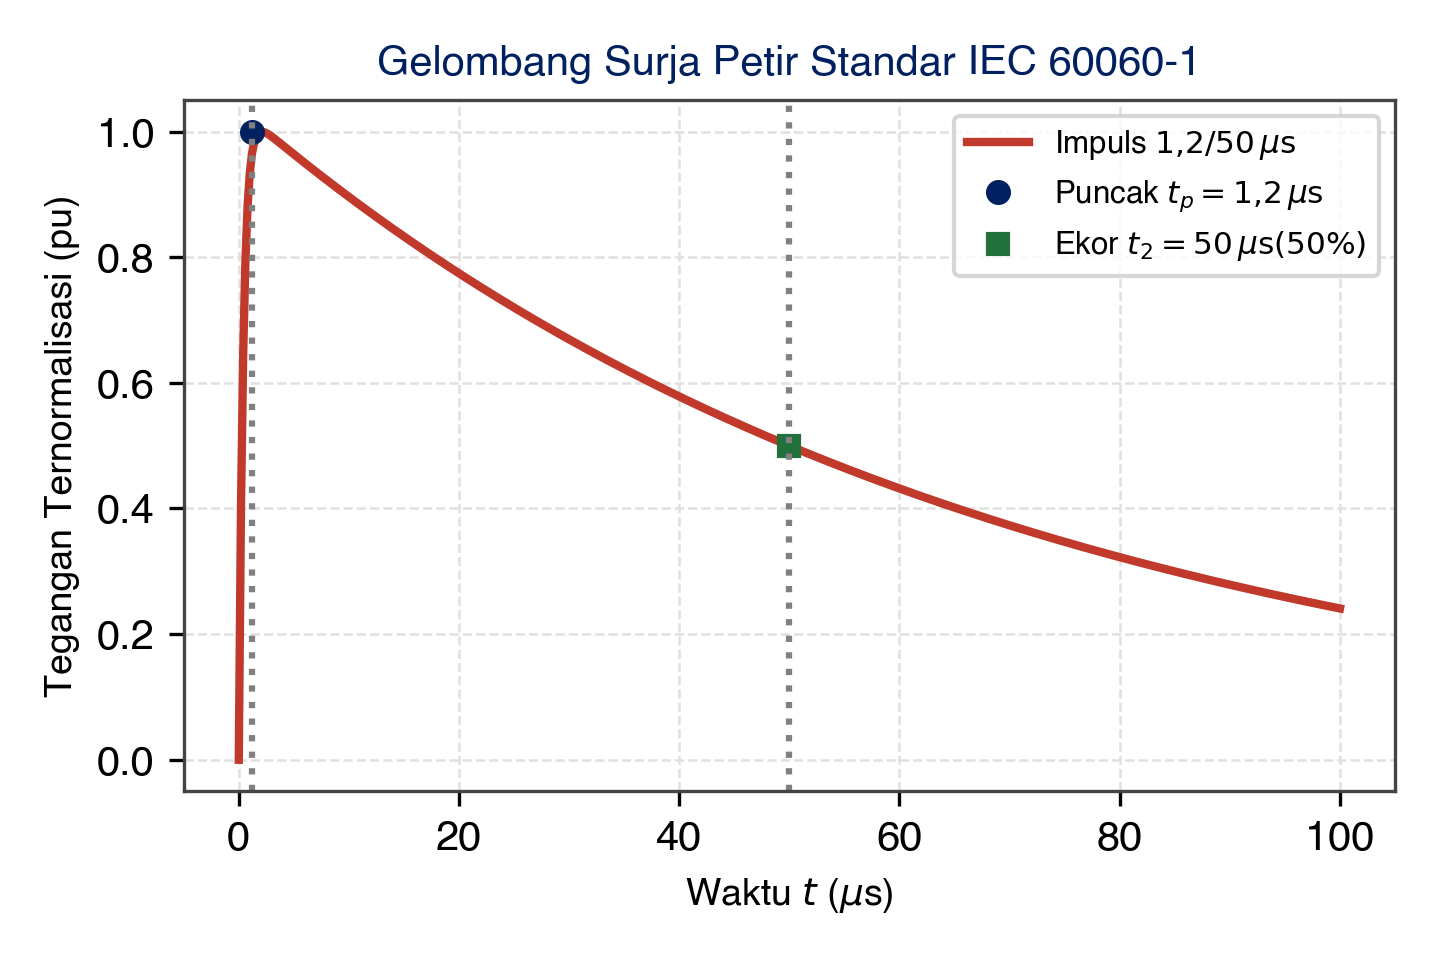
\includegraphics[width=\linewidth, height=0.38\textheight, keepaspectratio]{figures/slides/plot_ch6.png}
    \end{alertblock}
    \vspace{-0.1cm}
    \begin{exampleblock}{Intisari Gelombang Surja}
      \tiny
      Gelombang mencapai puncak dalam $1{,}2\,\mu\text{s}$ (laju kenaikan tinggi) dan meluruh ke $50\%$ pada $50\,\mu\text{s}$. Transformasi Laplace memungkinkan perhitungan respon isolator trafo secara eksak.
    \end{exampleblock}
  \end{columns}
\end{frame}

% FRAME 14: Kuis & Tantangan Bloom C1-C6
% FRAME 14: Kuis & Tantangan Bloom C1-C6
\begin{frame}{Kuis Konseptual Interaktif \& Evaluasi Bloom (C1--C6)}
  \begin{columns}[t]
    \column{0.52\textwidth}
    \begin{alertblock}{Peer Instruction: Uji Miskonsepsi Fisik}
      \footnotesize
      \textbf{Kasus Rekayasa:} Mengapa metode Transformasi Laplace $\mathcal{L}\{\cdot\}$ jauh lebih unggul daripada metode PDB klasik untuk menganalisis surja switching gardu induk?
      \vspace{0.05cm}
      \begin{itemize}\setlength{\itemsep}{1pt}
        \item \textbf{[A]} Laplace tidak memerlukan hukum tegangan Kirchhoff.
        \item \textbf{[B]} Laplace mengubah fungsi diskontinu (Heaviside/Dirac) dan turunan menjadi aljabar rasional domain-$s$ dengan kondisi awal otomatis!
        \item \textbf{[C]} Laplace hanya berlaku jika frekuensi bernilai nol.
        \item \textbf{[D]} Laplace meniadakan kebutuhan nilai induktansi.
      \end{itemize}
    \end{alertblock}

    \column{0.46\textwidth}
    \begin{block}{Tantangan Analisis \& Desain (C4--C6)}
      \footnotesize
      \begin{itemize}\setlength{\itemsep}{2pt}
        \item \textbf{C4 (Analisis):} Tentukan tegangan transien saat petir menyambar saluran dengan teorema geser waktu $e^{-as}$.
        \item \textbf{C5 (Evaluasi):} Buktikan Teorema Nilai Akhir $\lim_{t \to \infty} f(t) = \lim_{s \to 0} sF(s)$ pada transfer fungsi stabil.
        \item \textbf{C6 (Desain):} Rancang rangkaian pembentuk surja Marx Generator laboratorium uji tegangan tinggi!
      \end{itemize}
    \end{block}
  \end{columns}
\end{frame}

% FRAME 15: Rangkuman & Penutup
\begin{frame}{Rangkuman Inti Perkuliahan \& Referensi}
  \begin{exampleblock}{Intisari Perkuliahan Minggu 6}
    \begin{itemize}
      \item Transformasi Laplace mengonversi persoalan diferensial-integral domain-$t$ menjadi persamaan aljabar linier domain-$s$.
      \item Fungsi Heaviside $u(t)$ dan impuls Dirac $\delta(t)$ memungkinkan pemodelan sinyal pensaklaran diskontinu dan surja petir secara eksak.
      \item Teorema pergeseran pertama (translasi-$s$) dan kedua (translasi-$t$) merupakan kunci dalam menyederhanakan transformasi gelombang teredam dan tertunda.
    \end{itemize}
  \end{exampleblock}
  \vspace{0.2cm}
  \begin{center}
    \small \textbf{Buku Acuan Utama:} \\
    E. Kreyszig, \textit{Advanced Engineering Mathematics} | W. Hayt, \textit{Engineering Circuit Analysis}. \\
    \vspace{0.3cm}
    \textbf{Tautan Modul \& Bahan Ajar}: \url{https://pd.ndaratha.my.id} \\[0.12cm]\textbf{Video Kuliah (YouTube)}: {\color{red!85!black}\textbf{\url{https://youtu.be/iIYM-WRaTiU}}} \quad \textbar \quad \href{https://www.youtube.com/playlist?list=PLS5oOZWXZeTw}{\color{unibblue}\textbf{Playlist Lengkap}}
  \end{center}
\end{frame}

\end{document}
